\documentclass{article}
\usepackage{tikz}
\usetikzlibrary{shapes.geometric, arrows}
\usepackage[margin=1in]{geometry}

\begin{document}

\begin{figure}[h]
\centering
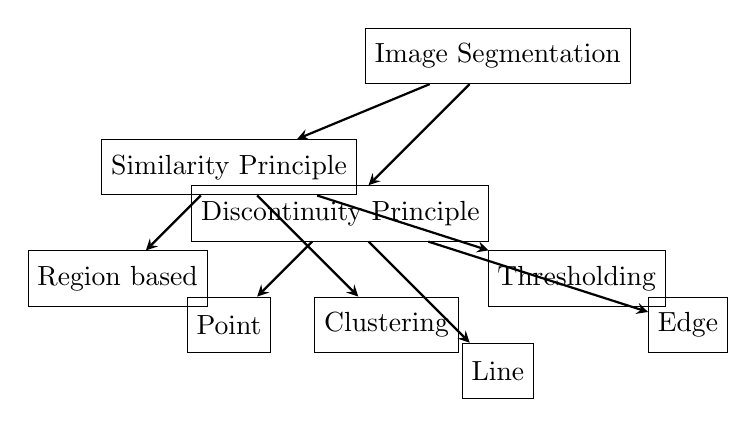
\begin{tikzpicture}[node distance=2cm]
\tikzstyle{box} = [rectangle, draw, text centered, minimum height=2em]
\tikzstyle{arrow} = [thick,->,>=stealth]

\node (seg) [box] {Image Segmentation};
\node (sim) [box, below left of=seg, xshift=-2cm] {Similarity Principle};
\node (dis) [box, below of=seg, xshift=-2cm] {Discontinuity Principle};

\node (point) [box, below left of=dis] {Point};
\node (line) [box, below of=dis, xshift=2cm] {Line};
\node (edge) [box, below right of=dis, xshift=3cm] {Edge};

\node (reg) [box, below left of=sim] {Region based};
\node (clus) [box, below of=sim, xshift=2cm] {Clustering};
\node (thres) [box, below right of=sim, xshift=3cm] {Thresholding};

\draw [arrow] (seg) -- (sim);
\draw [arrow] (seg) -- (dis);
\draw [arrow] (sim) -- (reg);
\draw [arrow] (sim) -- (clus);
\draw [arrow] (sim) -- (thres);
\draw [arrow] (dis) -- (point);
\draw [arrow] (dis) -- (line);
\draw [arrow] (dis) -- (edge);
\end{tikzpicture}
\caption{Overview of Image Segmentation Principles and Methods}
\label{fig:segmentation}
\end{figure}

\end{document} 